\begin{comment}
	Split data according to percentile
	RFCN resnet-101
	Pascal voc heavily skewed to smaller objects. Show plot
	50th percentile 13892.0
		test data also split according to this value
		cannot simply do by image basis - some images have multiple objects GTs - show figure
			total of 12275 GTs when doing this, still 3384 that are larger
		test images if only small images present - 697 images, 


	Results
		RFCN ResNet-101: 0.7632
		Model - 07++12 < 50th percentile
			All data: 0.5960
\end{comment}

\section{Resolution-Aware Object Detection}
Object detectors are commonly more accurate on objects that cover a larger number of pixels in an image. This is intuitive as objects with a lower resolution objectively have less details that can describe them. The poorer performance can be seen in \tableref{cocores}, for all object detectors the \gls{ap} is considerably lower for smaller objects in comparison to both medium and large. The best performing detector from \cite{deepres}, has an \gls{ap} difference of 35.3\%, from 50.9\% for large objects to 15.6\% for small. 
A potential method of tackling this issue is to train multiple detectors on separate partitions of the training data according to the size of the object. While deep-based \gls{cnn} have millions of parameters to generalise from training to testing, the difference between small and large objects may skew the learning towards the latter. In order to test this hypothesis an initial test will be conducted on the \gls{pascalvoc} dataset. However, \gls{pascalvoc} does not have the same definition of objects sizes as in \gls{mscoco}. Therefore, the distribution of the bounding boxes from the training set must be analysed in order to determine an appropriate split of data based on object size. This was done by parsing all of the bounding box coordinates in the 07++12 training set and calculating the area. A histogram of the area can be seen in \figref{0712hist}. There is a clear tendency to smaller objects in the training set with a clear skew towards the left of the figure.

\begin{figure}[H]
  \centering
    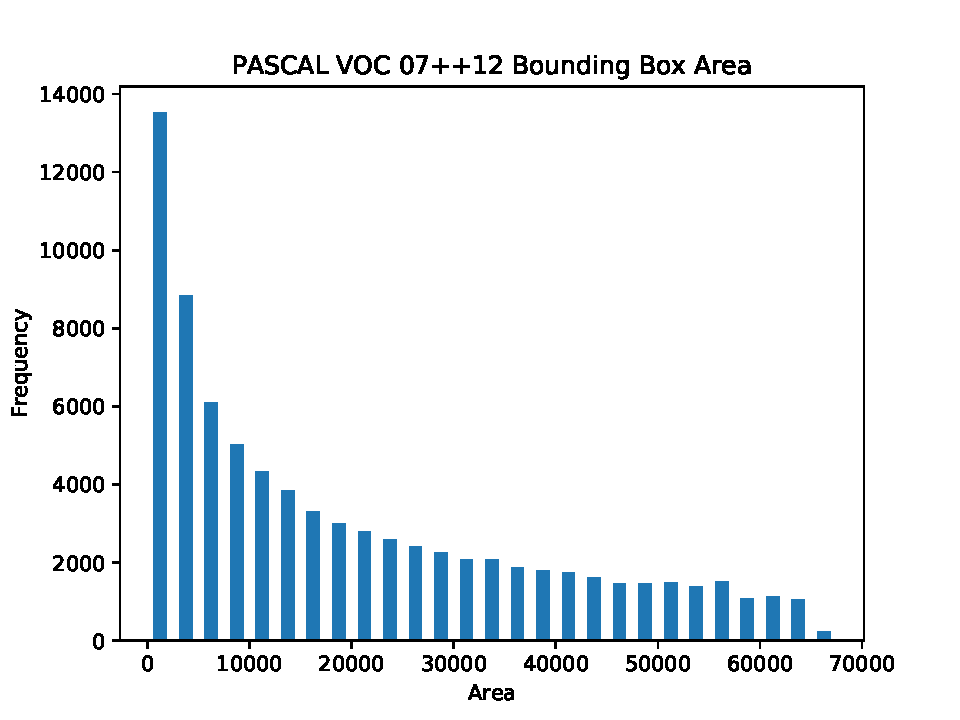
\includegraphics[width=0.6\textwidth]{Figs/Implementation/0712hist.pdf}
      \caption{Histogram of the \gls{pascalvoc} 07++12 bounding box area.}
    \label{fig:0712hist}
\end{figure}

As there is no clear way to split the data into three sets with equal amounts of data, the split was instead done into into two sets, one for small objects and another for larger. The split was made at the median bounding box area which is 13,892 pixels. Therefore, the dataset with bounding box area less than 13,982 pixels is denoted 07++12$_{small}$ and objects larger make up the dataset 07++12$_{larger}$.

Identical \gls{rfcn} with ResNet-101 networks were trained on either sets of data. Additionally the exact same training strategies were used in both instances which are outlined in \tableref{resawareparams}.

\begin{table}[h]
\centering
\caption{Learning parameters for the set of resolution-aware \gls{rfcn} object detectors.}
\label{tab:resawareparams}
\begin{tabular}{|l|l|}
\hline
\textbf{Parameter}            & \textbf{Value}  \\ \hline
base learning rate   & 0.001  \\ \hline
learning rate policy & step   \\ \hline
gamma                & 0.1    \\ \hline
stepsize             & 80,000 \\ \hline
momentum             & 0.9    \\ \hline
weight decay         & 0.0005 \\ \hline
\end{tabular}
\end{table}

Testing was done on the 07 test set but also split according to the median threshold found in the training data. The two testing sets are denoted as 07Test$_{small}$ and 07Test$_{larger}$. The size of the two test sets are 7,827 and 7,149 ground truth bounding boxes respectively. Histogram for the sets can be seen in \figref{smalltesthist} and \figref{largetesthist}.


\begin{figure}[H]
    \centering
    \begin{subfigure}[b]{0.45\textwidth}
        \center
        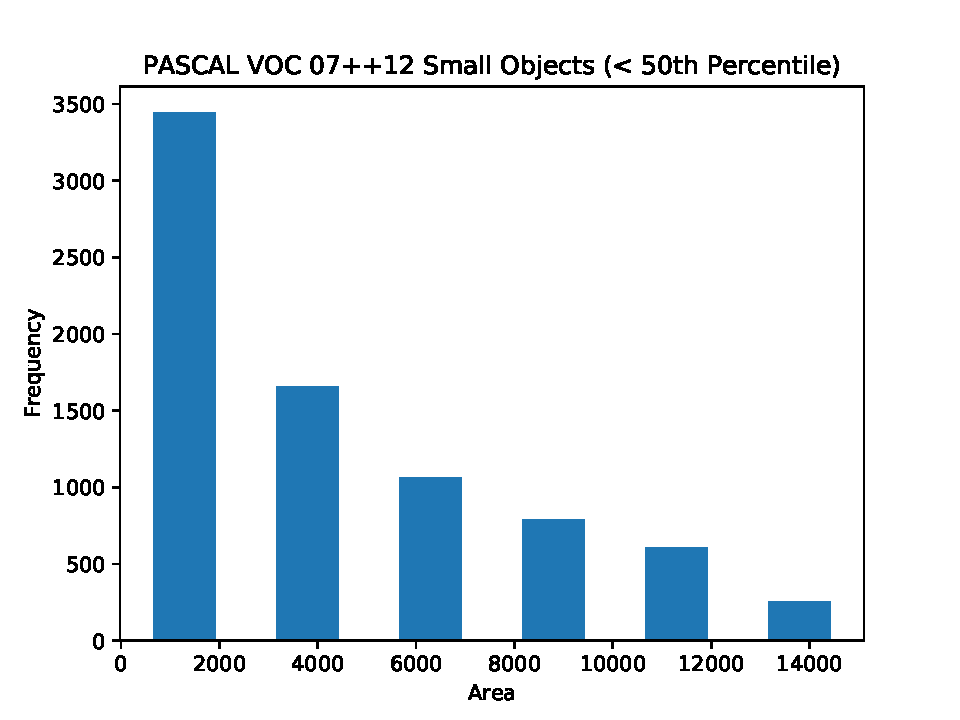
\includegraphics[width=\textwidth]{Figs/Implementation/testsmallhist.pdf}
        \caption{}\label{fig:smalltesthist}
    \end{subfigure}
    \begin{subfigure}[b]{0.45\textwidth}
        \center
        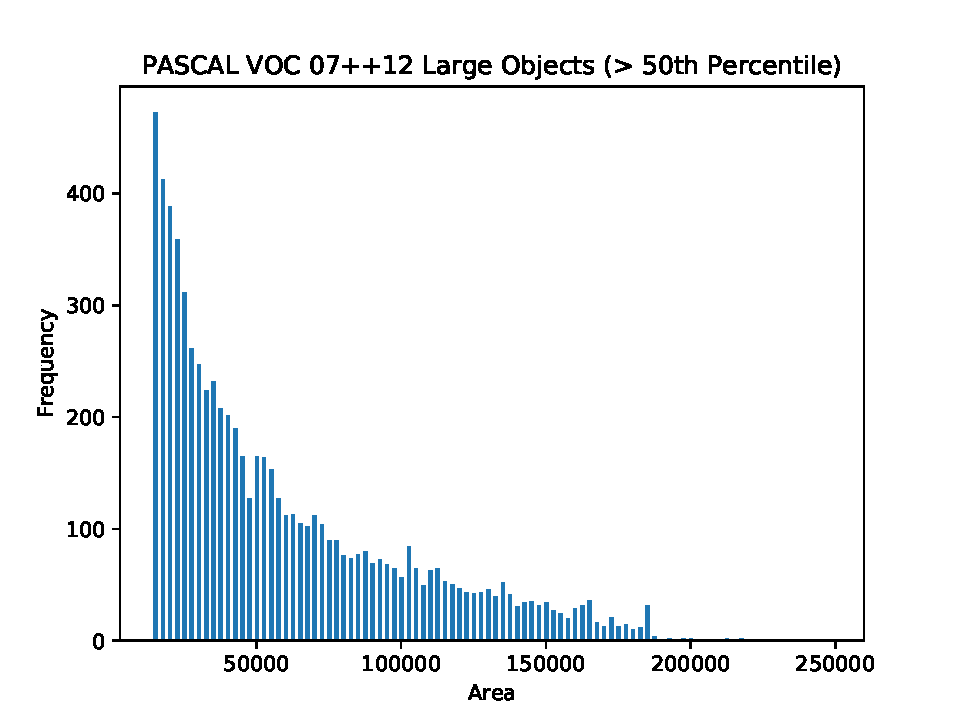
\includegraphics[width=\textwidth]{Figs/Implementation/testlargehist.pdf}
        \caption{}\label{fig:largetesthist}
    \end{subfigure}
    \caption{}
    \label{}
\end{figure} 

The results for the object detectors trained on the separate partitions of training data and a the baseline detector trained on all the data against the three sets of tests can be seen in \tableref{resresults}. The table shows that the detectors trained on the same relative size of data perform best.


\begin{table}[h]
\centering
\caption{Results}
\label{tab:resresults}
\begin{tabular}{|l|l|l|}
\hline
\textbf{Train Data}    & \textbf{Test Data}     & \textbf{mAP} \\ \hline
07++12$_{small}$ & 07Test$_{small}$  & \textbf{0.3410}   \\ \hline
07++12$_{larger}$  & 07Test$_{small}$ & 0.0308     \\ \hline
07++12   & 07Test$_{small}$           & 0.2216    \\ \hline
07++12$_{small}$ & 07Test$_{larger}$  &  0.3640   \\ \hline
07++12$_{larger}$ & 07Test$_{larger}$ &  \textbf{0.7660}   \\ \hline
07++12 & 07Test$_{larger}$           &  0.6434   \\ \hline
07++12$_{small}$       & 07   & 0.6265    \\ \hline
07++12$_{larger}$       & 07  &  0.5965   \\ \hline
07++12        & 07            &  \textbf{0.7635}   \\ \hline 
\end{tabular}
\end{table}